\documentclass[12pt, a4paper, twoside]{report}
\usepackage[utf8]{inputenc}
\usepackage{graphicx}
\usepackage[parfill]{parskip}
\usepackage{natbib}




\title{Tidynamics (CMSC6950)}
\author{Atiyeh Tahavorgar }
\date{June 2021}


\begin{document}
\maketitle
\section{Introduction}
A helpful reference for tidynamics is \cite{deBuyl2018}
\bibliographystyle{apalike}
\bibliography{bibliography.bib}\newpage
%\begin{tikzpicture}
%[remember picture, overlay] \draw[line width=1pt] ($(current page.north %west)+(1in,-0.5in)$) rectangle $(current page.south east)+(-0.5in,1in)$); 




%\section{About software}


In this report I explain about \textbf{software}, scientific problems solved by the software. Also, \textbf{computational tasks} and related \textbf{visualizations} will be explained. At the end of the report bibliography is added. 
\newpage
\section{software}
Tidynamics is a package to compute the dynamics of stochastic and molecular simulations with Fast Correlation Algorithm (FCA).tidynamics is designed as a library in which every routine operates directly on NumPy
arrays and returns NumPy arrays The goal of tidynamics is to serve as a reference implementation with a lighter interface. This package computes the followings:


Autocorrelation (the correlation of a time series with itself) 
The correlation between two time-series
\newline The mean-square displacement of a trajectory   
\newline  The cross-displacement (for off-diagonal realisations of Brownian motion)


There is a lack of a self-contained implementation of the algorithm. The software nMoldyn (Hinsen, Pellegrini, Stachura,  Kneller, 2012) implements it within a larger library but it has a more complex interface and more dependencies. The goal of tidynamics is to serve as a reference implementation with a lighter interface. 

tidynamics is designed as a library in which every routine operates directly on NumPy
arrays and returns NumPy arrays. The interface is simple and enables convenient use in
interactive sessions or in teaching material.

The Fast Correlation Algorithm relies on the Fourier transform to compute correlations.
For this purpose, we use NumPy’s (T. E. Oliphant, 2007) FFT module np.fft. The
advantage of using Fourier transforms is a reduced computational cost in comparison to a
direct loop over the data. We expect a scaling of the CPU time tCPU of tCPU ∝ N log N
where N is the length of the time series. We show in Figure 3 the actual CPU time and
compare it favourably to the expected scaling in the example Scaling behaviour.

NumPy (T. E. Oliphant, 2007) and SciPy (Jones, Oliphant, Peterson, & others, 2001)
implement correlation routines as well. In the case of NumPy, the computation is based
on a direct loop with a quadratic scaling of the CPU time O(N2
). In SciPy, both the
direct and a Fourier transform version are implemented.

The definition of np.correlate and scipy.signal.correlate differs from the definition
traditionally used in dynamical systems in two ways. These routines do not correct for
aperiodic signals, an issue that is addressed in the Fast Correlation Algorithm by zeropadding the signal, and they do not normalise the result by the actual number of samples.
In addition to these differences, the relative complexity of building SciPy and its larger
size motivated us to rely on NumPy only. NumPy and SciPy do not provide functions to
compute the mean-square displacement of trajectories. The Fast Correlation Algorithm
as applied to mean-square displacements was proposed by G. R. Kneller et al. (1995) and
is less known than the plain correlation algorithm.
The benefits of using tidynamics originate in the implementation of the suitable definitions
for the study of dynamical systems, good performance, and its ease of installation.


\newpage
\section{computational tasks}
In this project, I implement two computational tasks with two different visualization.


\subsection{tidynamics.correlation(data1, data2)}

Correlation between the input data using the Fast Correlation Algorithm. It has two  input signal with the same shape (N) and returns ndarray with the correlation for two inputs and the lag in units of the timestep in the input data. The correlation is given from time -N to time N.

 \textbf{Below is the code and its visualization for tidynamics.correlation(data1, data2)}:
\subsubsection{computation}

import matplotlib.pyplot as plt\newline
import pandas as pd\newline
import numpy as np\newline
import tidynamics\newline
plt.style.use('ggplot')\newline
font1 = ['family':'serif','color':'blue','size':20]\newline
font2 = ['family':'serif','color':'darkred','size':15]\newline

plt.rcParams['figure.figsize']=(10,10)\newline


spacing = np.linspace(-5 * np.pi, 5 * np.pi, num=500)\newline
t = np.linspace(-7 * np.pi, 7 * np.pi, num=500)\newline
s = pd.Series(0.6 * np.random.rand(500) + 0.3 * np.sin(spacing))\newline
t= pd.Series(0.4 * np.random.rand(500) + 0.7 * np.sin(spacing))\newline
acf = tidynamics.correlation(s,t)\newline



plt.plot(acf,marker='.',ms = 2, mfc = 'm',linestyle='dotted',linewidth = '2')\newline

plt.title("correlation over time",fontdict=font2,loc = 'right')\newline
plt.xlabel("correlation",fontdict=font1)\newline
plt.ylabel("time",fontdict=font1)\newline

plt.savefig("figure-correlaion.png", dpi=100, bbox_inches='tight')\newline
plt.show()\newline

\subsubsection{visualization}

\begin{center}
    \centering
    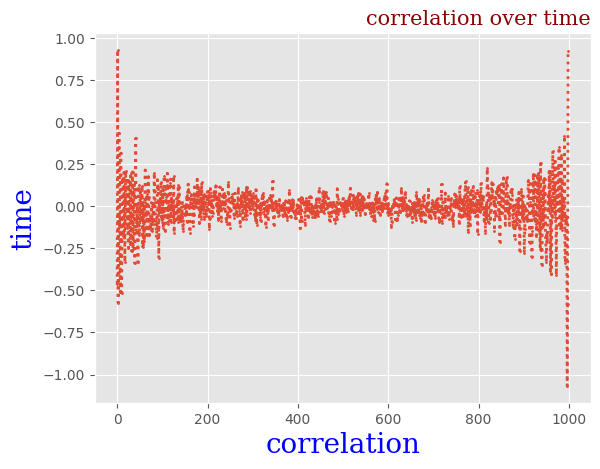
\includegraphics[width=1.1\textwidth , height=.6\paperheight]{figure_correlaion.png}
    \caption{correlation}
\end{center}

\newpage
\subsection{tidynamics.msd(pos)}

Mean-squared displacement (MSD) of the input trajectory using the Fast Correlation Algorithm.
Computes the MSD for all possible time deltas in the trajectory. The numerical results for large time deltas contain fewer samples than for small time times and are less accurate. This is intrinsic to the computation and not a limitation of the algorithm.\newline
It contains The input trajectory, of shape (N,) or (N,D) and returns ndarray of shape (N,) with the MSD for successive linearly spaced time delays.

\textbf{Below is the code and its visualization for tidynamics.msd(pos)}:
\subsubsection{computation}
\small

import array as arr\newline
import matplotlib.pyplot as plt\newline
import tidynamics\newline
import random\newline
import sys\newline
from numpy import *\newline

font1 = {'family':'serif','color':'blue','size':20}\newline
font2 = {'family':'serif','color':'darkred','size':15}\newline


plt.rcParams['figure.figsize']=(10,10)\newline

plt.style.use('Solarize-Light2')\newline



try:\newline
    N=3000\newline
    mean=linspace(0,0,N,dtype=float)\newline
    count=0\newline
    dock=range(1,100)\newline
    for i in dock:\newline\newline
        s=[-1,1]\newline
        steps=random.choice(s, size=(N,2))\newline
        data = cumsum(steps, axis=0)\newline
         mean += tidynamics.msd(data)\newline
        count+=1\newline


    mean /= count\newline
    mean = mean[1:N//2]\newline

    T = arange(1,N//2)\newline

    plt.plot(T, mean,color="#444444",linestyle="--",marker = 'o',ms =5 ,linewidth = '1', label='Random walk (num.)')\newline

    plt.plot(T, 2*l,color="r",linestyle="--",marker = 'o',ms =5,linewidth = '1', label='Random walk (theo.)')\newline

    plt.plot(T[1:], tidynamics.msd(l)[1:],color="#bf00ff", marker='o', ms = 5,linewidth = '1',label='Constant velocity )\newline    plt.plot(l[1:], l[1:]**2,color="#eeb704", marker='o' ,ms = 5,linewidth = '1', label='Constant velocity (theo.)')\newline

    plt.legend()\newline
    plt.loglog()\newline\newline
    plt.plot()\newline
    plt.xlabel('time', fontdict = font1, fontsize=10)\newline
    plt.ylabel('mean square displacement',fontdict = font1, fontsize=10)\newline
    plt.title('Examples for the mean-square displacement', fontdict = font2, fontsize=10, loc = 'left')\newline
    plt.savefig("figure_msd.png", dpi=100, bbox_inches='tight')\newline
    plt.show()\newline
    \newpage
    \subsubsection{visualization}

\begin{center}
    \centering
    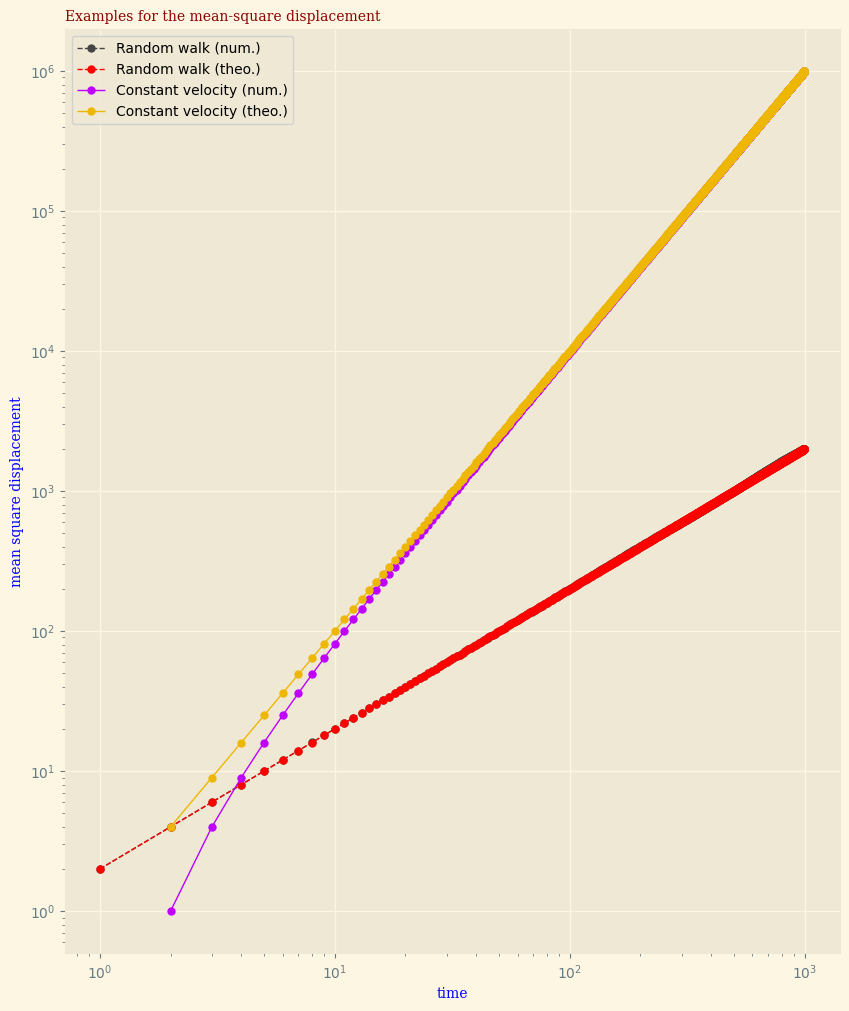
\includegraphics[width=1.1\textwidth , height=.6\paperheight]{figure_msd.png}
    \caption{correlation}
\end{center}

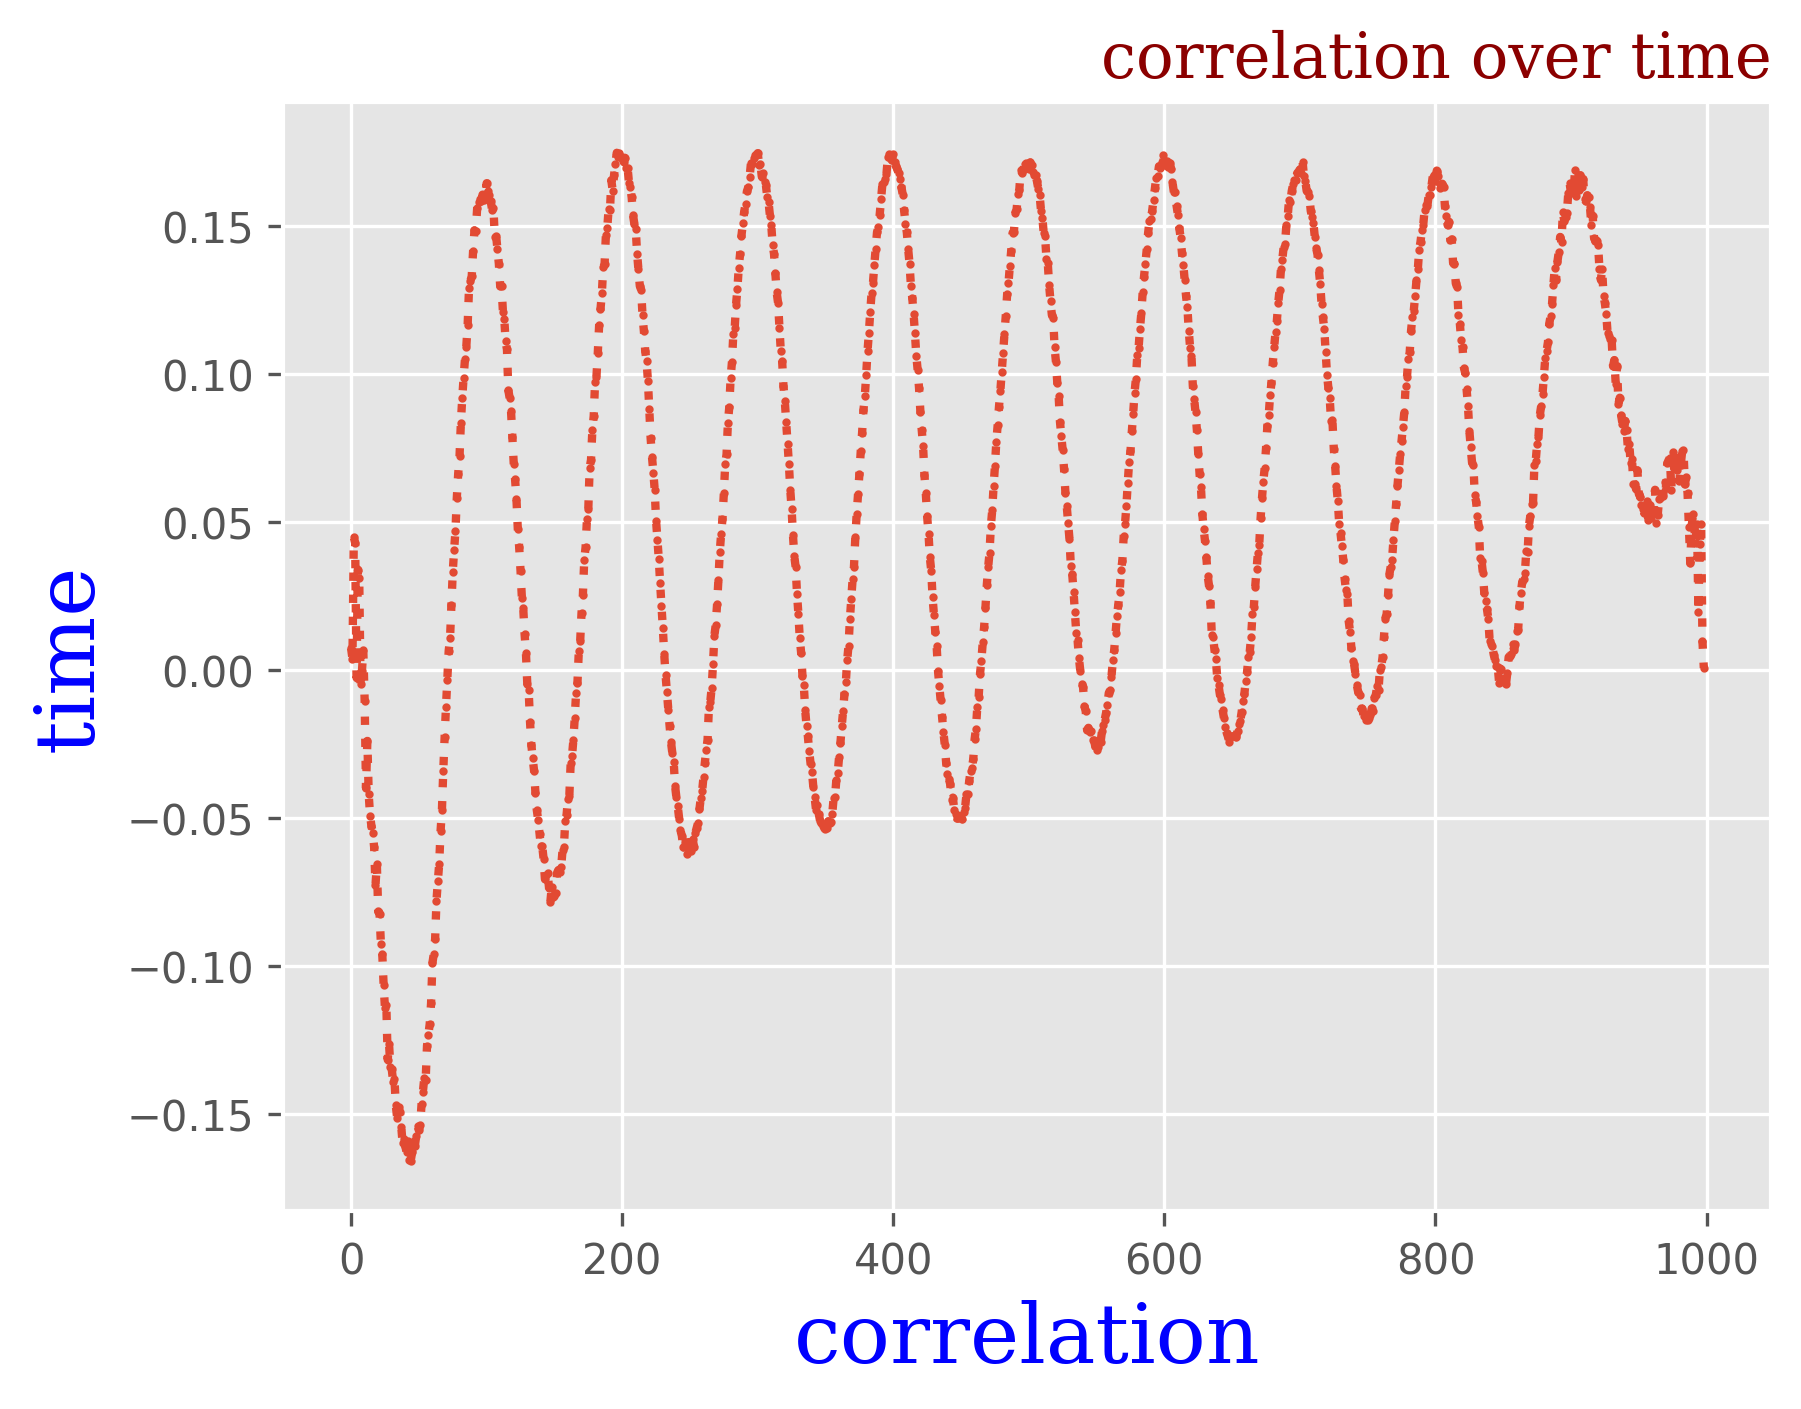
\includegraphics{figure_correlation}

\end{document}
